% Für Bindekorrektur als optionales Argument "BCORfaktormitmaßeinheit", dann
% sieht auch Option "twoside" vernünftig aus
% Näheres zu "scrartcl" bzw. "scrreprt" und "scrbook" siehe KOMA-Skript Doku
\documentclass[12pt,a4paper,titlepage,headinclude,bibtotoc]{scrartcl}


%---- Allgemeine Layout Einstellungen ------------------------------------------

% Für Kopf und Fußzeilen, siehe auch KOMA-Skript Doku
\usepackage[komastyle]{scrpage2}
\pagestyle{scrheadings}
\automark[section]{chapter}
\setheadsepline{0.5pt}[\color{black}]

%keine Einrückung
\parindent0pt

%Einstellungen für Figuren- und Tabellenbeschriftungen
\setkomafont{captionlabel}{\sffamily\bfseries}
\setcapindent{0em}


%---- Weitere Pakete -----------------------------------------------------------
% Die Pakete sind alle in der TeX Live Distribution enthalten. Wichtige Adressen
% www.ctan.org, www.dante.de

% Sprachunterstützung
\usepackage[ngerman]{babel}

% Benutzung von Umlauten direkt im Text
% entweder "latin1" oder "utf8"
\usepackage[utf8]{inputenc}

% Pakete mit Mathesymbolen und zur Beseitigung von Schwächen der Mathe-Umgebung
\usepackage{latexsym,exscale,amssymb,amsmath}

% Weitere Symbole
\usepackage[nointegrals]{wasysym}
\usepackage{eurosym}

% Anderes Literaturverzeichnisformat
%\usepackage[square,sort&compress]{natbib}

% Für Farbe
\usepackage{color}

% Zur Graphikausgabe
%Beipiel: \includegraphics[width=\textwidth]{grafik.png}
\usepackage{graphicx}

% Text umfließt Graphiken und Tabellen
% Beispiel:
% \begin{wrapfigure}[Zeilenanzahl]{"l" oder "r"}{breite}
%   \centering
%   \includegraphics[width=...]{grafik}
%   \caption{Beschriftung} 
%   \label{fig:grafik}
% \end{wrapfigure}
\usepackage{wrapfig}

% Mehrere Abbildungen nebeneinander
% Beispiel:
% \begin{figure}[htb]
%   \centering
%   \subfigure[Beschriftung 1\label{fig:label1}]
%   {\includegraphics[width=0.49\textwidth]{grafik1}}
%   \hfill
%   \subfigure[Beschriftung 2\label{fig:label2}]
%   {\includegraphics[width=0.49\textwidth]{grafik2}}
%   \caption{Beschriftung allgemein}
%   \label{fig:label-gesamt}
% \end{figure}
\usepackage{subfigure}

% Caption neben Abbildung
% Beispiel:
% \sidecaptionvpos{figure}{"c" oder "t" oder "b"}
% \begin{SCfigure}[rel. Breite (normalerweise = 1)][hbt]
%   \centering
%   \includegraphics[width=0.5\textwidth]{grafik.png}
%   \caption{Beschreibung}
%   \label{fig:}
% \end{SCfigure}
\usepackage{sidecap}

% Befehl für "Entspricht"-Zeichen
\newcommand{\corresponds}{\ensuremath{\mathrel{\widehat{=}}}}

%Für chemische Formeln (von www.dante.de)
%% Anpassung an LaTeX(2e) von Bernd Raichle
\makeatletter
\DeclareRobustCommand{\chemical}[1]{%
  {\(\m@th
   \edef\resetfontdimens{\noexpand\)%
       \fontdimen16\textfont2=\the\fontdimen16\textfont2
       \fontdimen17\textfont2=\the\fontdimen17\textfont2\relax}%
   \fontdimen16\textfont2=2.7pt \fontdimen17\textfont2=2.7pt
   \mathrm{#1}%
   \resetfontdimens}}
\makeatother

%Si Einheiten
\usepackage{siunitx}

%c++ Code einbinden
\usepackage{listings}
\lstset{numbers=left, numberstyle=\tiny, numbersep=5pt}

%Differential
\newcommand{\dif}{\ensuremath{\mathrm{d}}}

%Boxen,etc.
\usepackage{fancybox}
\usepackage{empheq}

%Fußnoten auf gleiche Seite
\interfootnotelinepenalty=1000

%Bibliography \bibliography{literatur} und \cite{gerthsen}
%\usepackage{cite}
\usepackage{babelbib}
\selectbiblanguage{ngerman}


\begin{document}

\begin{titlepage}
\centering
\textsc{\Large Anfängerpraktikum der Fakultät für
  Physik,\\[1.5ex] Universität Göttingen}

\vspace*{4.2cm}

\rule{\textwidth}{1pt}\\[0.5cm]
{\huge \bfseries
  Dampfdruck von Wasser\\[1.5ex]
  Protokoll:}\\[0.5cm]
\rule{\textwidth}{1pt}

\vspace*{3.0cm}

\begin{Large}
\begin{tabular}{ll}
Praktikant:
%	&  Skrollan Detzler\\
 	&  Felix Kurtz\\
 	&  Michael Lohmann\\
%	&  Kevin Lüdemann\\

  E-Mail: 
%	&  skrollan.detzler@stud.uni-goettingen.de\\
	&  felix.kurtz@stud.uni-goettingen.de\\
	& m.lohmann@stud.uni-goettingen.de\\	
%	&  kevin.luedemann@stud.uni-goettingen.de\\

 Betreuer: & Martin Ochmann\\
 Versuchsdatum: & 23.06.2014\\
\end{tabular}
\end{Large}

\vspace*{0.8cm}

\begin{Large}
\fbox{
  \begin{minipage}[t][2.5cm][t]{6cm} 
    Testat:
  \end{minipage}
}
\end{Large}

\end{titlepage}

\tableofcontents

\newpage

\section{Einleitung}
\label{sec:einleitung}
%ein paar Sätze vorneweg
Ein \textit{Schnellkochtopf} basiert auf dem Prinzip des Dampfdrucks.
In ihm steigt der Druck an und somit erhöht sich die Siedetemperatur von Wasser und das Essen wird schneller gar.
Außerdem wird dadurch Energie gespart.
Um dies zu verstehen reicht das Ideale Gasmodell nicht mehr aus, sondern es muss eine genauere Näherung betrachtet werden.

\section{Theorie}
\label{sec:theorie}

\subsection{Van-der-Waals-Gleichung}
Die reale Gasgleichung lautet nach \cite[S. 303]{gerthsen} mit der Ersetzung von $V_\text{mol}=V/n$ 
\begin{align}
\left(p+\frac{n^2a}{V^2}\right)\left( V-nb \right)=nRT \label{eq:vanderwaalsgl}
\end{align}
Dabei betragen für Wasser die \emph{Van-der-Waals-Konstanten} $a=0.5537~\si{\pascal~\meter^6}$ (Binnendruck) und $b=3.05\cdot10^{-5}\si{\meter^3}$ (Sättigungsdruck).\\
Sie entsteht dadurch, dass bei realen Gasen die Ausdehnung der Atome nicht mehr vernachlässigt wird.
Dadurch ist das "reale Volumen" größer, als das ideale und zwar um eine stoffabhängige Konstante multipliziert mit der Stoffmenge: $V_\text{ideal}=V_\text{Real}-n\cdot b$ .\\
Da in der idealen Gasgleichung die intermolekularen Kräfte bis auf elastische Stöße vernachlässigt sind, muss auch im Druck ein Korrekturfaktor eingeführt werden.
Der Druck sinkt durch die zusätzlichen Möglichkeiten, Energie an andere Teilchen zu übertragen, weshalb zu dem ``realen Druck'' ein Summand hinzugefügt werden muss, um den idealen zu bekommen: $p_\text{ideal}=p_\text{real}+\frac{n^2\cdot a^2}{V^2}$ .
Aus der idealen Gasgleichung $p_\text{ideal}V_\text{ideal}=nRT$ wird so Gleichung \eqref{eq:vanderwaalsgl}.


\subsection{Maxwell'sche Gerade}
Diskutiert man die Kurven, die sich aus der Van-der-Waals-Gleichung ergeben, so stellt man leicht fest, dass die Kurven für hohe Temperaturen einer Hyperbel entsprechen.
Für kleinere Temperaturen weicht die Kurve aber immer mehr von der Hyperbel ab (s. Abb. \ref{fig:vanderwaalskurven}) und unterhalb einer kritischen Temperatur $T_k$ besitzt sie sogar zwei Extrempunkte.
Da ein Gas somit bei einer Temperatur einen bestimmten Druck bei mehreren Volumina annehmen kann, könnte man damit ein \emph{Perpetuum Mobile} 2. Art bauen.
Der 2. Hauptsatz der Thermodynamik verbietet dies jedoch und so führte Maxwell eine Korrekturgerade für diesen Bereich ein.
Er forderte, dass eine waagerechte Gerade so in diesen Bereich eingepasst wurde, dass der Flächeninhalt zwischen Gerade und Van-der-Waals-Gleichung in beiden Abschnitten gleich groß ist.
Diese Gerade erhielt ihm zu ehren den Namen \emph{Maxwell Gerade}.
Befindet sich das Gas auf diesem Abschnitt, so bleibt sein Druck konstant, obwohl sein Volumen sich verändert.
Es muss also ein Teil des Stoffes vom festen in den flüssigen Aggregatzustand übergehen (oder umgekehrt).
Dies geschieht so lange, bis der Sättigungsdampfdruck $p_S$ erreicht ist, welcher der Höhe der Geraden entspricht.
Mit sinkender Temperatur sinkt auch der Dampfdruck und die Maxwell-Gerade wird länger.
%%%%%%%%%%%%%%%%%%%%%%%%%%%%%%%%%%%%%%%%Bild mit Van-der-Waals-Kurven
\begin{figure}[!h]
\centering
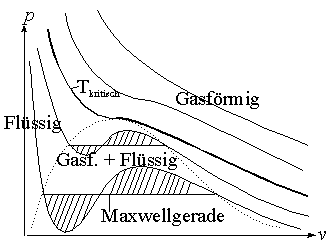
\includegraphics[scale=0.6]{vanwaalsiso}
\caption{Darstellung verschiedener Isotherme aus der Van-der-Waals-Gleichung von \protect\footnotemark}
\label{fig:vanderwaalskurven}
\end{figure}
\footnotetext{30.08.2014, 16:00 Uhr, http://www.physikon.de/01/14/01van3.gif} 
\subsection{Carnot'scher Kreisprozess}
Ein Carnot'scher Kreisprozess ist in 4 Schritte geteilt.
\begin{itemize}
\item $1\rightarrow 2$: isotherme Expansion, bei der die Wärme $Q_C$ hinzugeführt wird.
\item $2\rightarrow 3$: adiabatische Expansion, bei der eine Abkühlung von der Temperatur $T_A$ auf $T_B$ stattfindet.
\item $3\rightarrow 4$: isotherme Kompression, durch Wärmeentzug von $Q_D$ auf dem Temperaturniveau $T_B$.
\item $4\rightarrow 1$: adiabatische Kompression bis der Anfangszustand wieder erreicht ist.
	Ein Carnot-Prozess ist also ein Prozess, an dessen Ende im System wieder die Ausgangslage ist.
\end{itemize}
Die geleistete Arbeit in diesem Prozess bestimmt sich aus der Größe der eingeschlossenen Fläche im $p$-$V$-Diagramm.
Da sie größer wird, je größer der Temperaturunterschied $T_A-T_B$ ist, ist auch somit der Wirkungsgrad hierbei größer.

\newpage
\subsection{Clausius-Clapeyron-Gleichung}
\begin{figure}[!h]
\centering
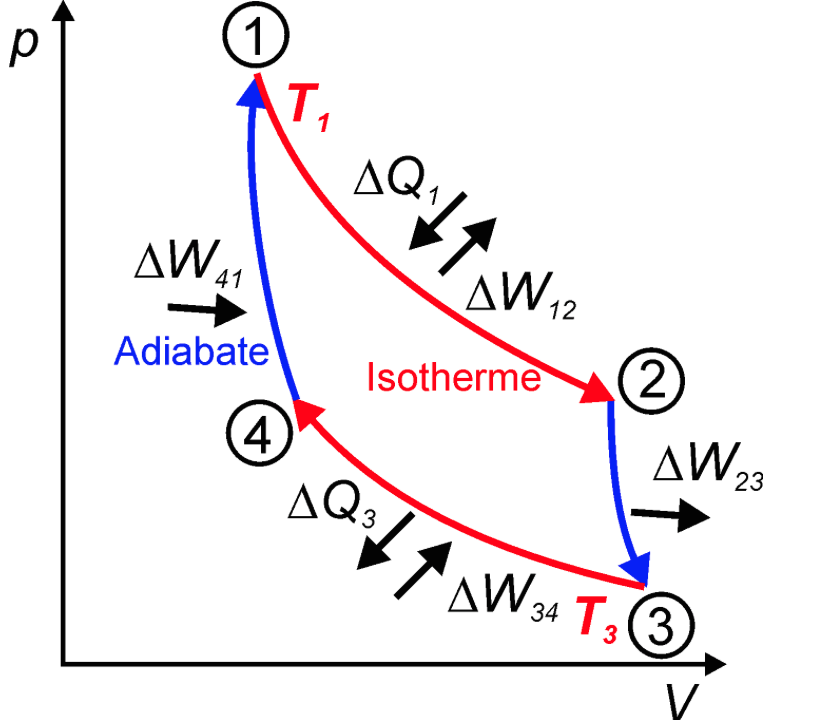
\includegraphics[scale=0.3]{Carnot}
\caption{Darstellung des Carnot-Prozesses nach \protect\footnotemark}
\label{fig:carnot}
\end{figure}
\footnotetext{http://www.ipf.uni-stuttgart.de/lehre/online-skript/waerme/carnot.gif}
Man kann sich nun einen Carnot-Prozess vorstellen, bei dem in einem Zylinder mit Kolben abwechselnd Wasser verdampft und kondensiert wird.
Dieser beginnt mit einer komplett kondensierten Gasphase an Punkt 1 bei einer Temperatur von $T+dT$.
$1\rightarrow 2$ ist eine Isotherme nach der Van-der-Waals-Gleichung.
Die verrichtete Arbeit ist% unter Zufuhr der Verdampfungsenergie $\Lambda$
\begin{align*}
\Delta W_{12}=-(p+dp)(V_\text D-V_\text{Fl})
\end{align*}
Wobei die Wärmezufuhr einerseits die Arbeit $-\Delta W_{12}$ verrichtet, andererseits aber auch die Flüssigkeit verdampft.
2 ist nun der Punkt, an dem die komplette Flüssigkeit verdampft ist.
Die adiabatische Expansion $2\rightarrow 3$ verursacht eine Abkühlung um $dT$.
Diese Temperatur wird nun in der isothermen Kompression erhalten, bis an Position 4 wieder aller Dampf kondensiert ist.\\
Durch die infinitesimale Temperaturänderung $dT$ können die Näherungen
\begin{align*}
V_\text D = V_{\text{D}_2}= V_{\text{D}_3}\qquad\text{und}\qquad V_\text{Fl}=V_{\text{Fl}_2}=V_{\text{Fl}_3}
\end{align*}
verwendet werden.
Außerdem sind dadurch die geleisteten Arbeiten $W_{23}$ und $W_{41}$ vernachlässigbar.
So wird in $3\rightarrow 4$ die Arbeit
\begin{align*}
\Delta W_{34}=p\cdot (V_\text D-V_\text{Fl})
\end{align*}
verrichtet.
Um wieder zum Ausgangspunkt 1 zurück zu kommen, muss das Volumen wieder um $dT$ erwärmt werden.\\
Die insgesamt geleistete Arbeit ist unter Vernachlässigung von $W_{23}$ und $W_{41}$
\begin{align*}
-\Delta W=-\Delta W_{12}-\Delta W_{34}=-dp\cdot (V_\text D -V_\text{Fl})
\end{align*}
Woraus sich mit der Formel für den Wirkungsgrad eines Carnot-Prozesses die Verdampfungswärme $\Lambda$ errechnen lässt:
\begin{align*}
\eta&=-\frac{\Delta W}{\Delta Q}=\frac{dp\cdot (V_\text D-V_\text{Fl})}{\Lambda}=\frac{dT}{T+dT}\approx \frac{dT}{T}\\
\Leftrightarrow\qquad \Lambda&=T\frac{dp}{dT}(V_\text D-V_\text{Fl})
\end{align*}
Hieraus kann nun mit dem idealen Gasgesetz unter Trennung der Variablen und mithilfe Integrierens die \emph{Dampfdruckformel} nach \cite[S. 342, Formel (10.127)]{demtroeder} hergeleitet werden
\begin{align}
p(T)=p_0\cdot \exp\left( \frac{\Lambda}{R}\cdot\left( \frac{1}{T_0}-\frac{1}{T} \right)\right)
\label{eq:Dampfdruck}
\end{align}



\subsection{Widerstandsthermometer}

Bei diesem Versuch wird zur Messung der Temperatur ein Pt1000-Widerstandsthermometer verwendet.
Der Name verrät, dass der Messfühler aus Platin ist und bei $0\si{\celsius}$ einen Widerstand von $R_0=1000\si{\ohm}$ hat.
Der Widerstand hängt so von der Temperatur $\vartheta>0\si{\celsius}$ ab:
\begin{align}
R(\vartheta)&=R_0\cdot\left(1 + A\vartheta + B\vartheta^2\right) \label{eq:Pt1000}
\end{align}
Die zugehörigen Konstanten findet man in Tabelle \ref{tab:Pt1000}.

\begin{table}[!htb]
\centering
\begin{tabular}{|c|c|}
\hline
R$_0$ & $1000 ~ \si{\ohm}$\\
A   & $3.9083 \cdot 10^{-3} ~ \si{\celsius^{-1}}$\\
B   & $-5.775 \cdot 10^{-7} ~ \si{\celsius^{-2}}$\\
\hline
\end{tabular}
\caption{Kennwerte des Widerstandsthermometers}
\label{tab:Pt1000}
\end{table}

Der Fehler der Temperaturmessung dieses Gerätes liegt bei
\begin{align}
\Delta\vartheta=\pm (0.3~\si{\celsius}+0.005\vartheta)~.
\label{eq:Pt1000_fehler}
\end{align}


\section{Durchführung}
\label{sec:durchfuehrung}
\begin{figure}[!htb]
\centering
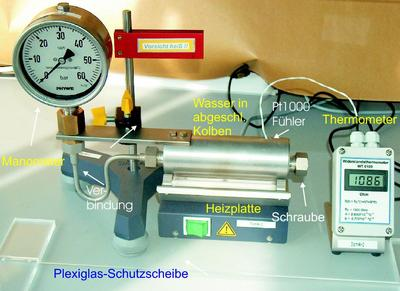
\includegraphics[scale=1.0]{Aufbau.jpg}
\caption{Versuchsaufbau Quelle:LP}	
\label{fig:Aufbau}
\end{figure}

Nachdem die Sicherheitshinweise (insbesondere die starke Erwärmung und der hohe Druck steigert das Gefahrenpotential) sorgfältig durchgelesen wurden, schaltet man das Gerät ein.
Der Heizstrahler erwärmt dann den mit Wasser gefüllten Kolben, welches dadurch verdampft.
Am angeschlossenen Manometer liest man den Druck ab.
Zeitgleich notiert man den Wert des Widerstandsthermometers und somit indirekt die Temperatur.
Dies geschieht in 1 Bar-Schritten.
Das Heizen wird beendet, wenn $1900 ~\si{\ohm}$ oder $45 \si{\bar}$ überschritten werden, damit das Gerät keinen Schaden nimmt.
Nun wird die Messung während des Abkühlens wiederholt.

\section{Auswertung}
\label{sec:auswertung}
\subsection{Druckkurven}
Löst man \eqref{eq:Pt1000} nach der Temperatur $\vartheta$ auf, ergibt sich folgende Gleichung
\begin{align}
	\vartheta&=-\frac{A}{2B}-\sqrt{\frac{A^2}{4B^2}-\frac{1}{B}+\frac{R}{R_0 B}}
\end{align}
Für den Fehler $\Delta\vartheta$ benutzt man \eqref{eq:Pt1000_fehler}.
Nun muss $\vartheta$ noch in Kelvin umgerechnet werden.
Außerdem wird für $p_0$ der gemessene Umgebungsdruck von 1017 hPa verwendet.
Trägt man nun den Druck logarithmisch gegen den Kehrwert der Temperatur auf, erwartet man nach \eqref{eq:Dampfdruck} eine Gerade $$\ln\left(\frac{p}{p_0}\right) = -\frac{\Lambda}{R}\cdot\frac{1}{T}+\frac{\Lambda}{R}\cdot \frac{1}{T_0} = m \cdot T^{-1} + b$$
Einen solchen Graphen nennt man \textit{Arrheniusplot}.
Dies wurde einmal für das Erwärmen (Abb. \ref{fig:mess1}) und das Abkühlen (Abb. \ref{fig:mess2}) gemacht, die Werte aus der linearen Regression finden sich in Tabelle \ref{tab:regErg} wieder.

\begin{figure}[!htb]
	\centering
	% GNUPLOT: LaTeX picture with Postscript
\begingroup
  \makeatletter
  \providecommand\color[2][]{%
    \GenericError{(gnuplot) \space\space\space\@spaces}{%
      Package color not loaded in conjunction with
      terminal option `colourtext'%
    }{See the gnuplot documentation for explanation.%
    }{Either use 'blacktext' in gnuplot or load the package
      color.sty in LaTeX.}%
    \renewcommand\color[2][]{}%
  }%
  \providecommand\includegraphics[2][]{%
    \GenericError{(gnuplot) \space\space\space\@spaces}{%
      Package graphicx or graphics not loaded%
    }{See the gnuplot documentation for explanation.%
    }{The gnuplot epslatex terminal needs graphicx.sty or graphics.sty.}%
    \renewcommand\includegraphics[2][]{}%
  }%
  \providecommand\rotatebox[2]{#2}%
  \@ifundefined{ifGPcolor}{%
    \newif\ifGPcolor
    \GPcolortrue
  }{}%
  \@ifundefined{ifGPblacktext}{%
    \newif\ifGPblacktext
    \GPblacktexttrue
  }{}%
  % define a \g@addto@macro without @ in the name:
  \let\gplgaddtomacro\g@addto@macro
  % define empty templates for all commands taking text:
  \gdef\gplbacktext{}%
  \gdef\gplfronttext{}%
  \makeatother
  \ifGPblacktext
    % no textcolor at all
    \def\colorrgb#1{}%
    \def\colorgray#1{}%
  \else
    % gray or color?
    \ifGPcolor
      \def\colorrgb#1{\color[rgb]{#1}}%
      \def\colorgray#1{\color[gray]{#1}}%
      \expandafter\def\csname LTw\endcsname{\color{white}}%
      \expandafter\def\csname LTb\endcsname{\color{black}}%
      \expandafter\def\csname LTa\endcsname{\color{black}}%
      \expandafter\def\csname LT0\endcsname{\color[rgb]{1,0,0}}%
      \expandafter\def\csname LT1\endcsname{\color[rgb]{0,1,0}}%
      \expandafter\def\csname LT2\endcsname{\color[rgb]{0,0,1}}%
      \expandafter\def\csname LT3\endcsname{\color[rgb]{1,0,1}}%
      \expandafter\def\csname LT4\endcsname{\color[rgb]{0,1,1}}%
      \expandafter\def\csname LT5\endcsname{\color[rgb]{1,1,0}}%
      \expandafter\def\csname LT6\endcsname{\color[rgb]{0,0,0}}%
      \expandafter\def\csname LT7\endcsname{\color[rgb]{1,0.3,0}}%
      \expandafter\def\csname LT8\endcsname{\color[rgb]{0.5,0.5,0.5}}%
    \else
      % gray
      \def\colorrgb#1{\color{black}}%
      \def\colorgray#1{\color[gray]{#1}}%
      \expandafter\def\csname LTw\endcsname{\color{white}}%
      \expandafter\def\csname LTb\endcsname{\color{black}}%
      \expandafter\def\csname LTa\endcsname{\color{black}}%
      \expandafter\def\csname LT0\endcsname{\color{black}}%
      \expandafter\def\csname LT1\endcsname{\color{black}}%
      \expandafter\def\csname LT2\endcsname{\color{black}}%
      \expandafter\def\csname LT3\endcsname{\color{black}}%
      \expandafter\def\csname LT4\endcsname{\color{black}}%
      \expandafter\def\csname LT5\endcsname{\color{black}}%
      \expandafter\def\csname LT6\endcsname{\color{black}}%
      \expandafter\def\csname LT7\endcsname{\color{black}}%
      \expandafter\def\csname LT8\endcsname{\color{black}}%
    \fi
  \fi
  \setlength{\unitlength}{0.0500bp}%
  \begin{picture}(7200.00,5040.00)%
    \gplgaddtomacro\gplbacktext{%
      \csname LTb\endcsname%
      \put(946,704){\makebox(0,0)[r]{\strut{}-0.5}}%
      \put(946,1156){\makebox(0,0)[r]{\strut{} 0}}%
      \put(946,1609){\makebox(0,0)[r]{\strut{} 0.5}}%
      \put(946,2061){\makebox(0,0)[r]{\strut{} 1}}%
      \put(946,2513){\makebox(0,0)[r]{\strut{} 1.5}}%
      \put(946,2966){\makebox(0,0)[r]{\strut{} 2}}%
      \put(946,3418){\makebox(0,0)[r]{\strut{} 2.5}}%
      \put(946,3870){\makebox(0,0)[r]{\strut{} 3}}%
      \put(946,4323){\makebox(0,0)[r]{\strut{} 3.5}}%
      \put(946,4775){\makebox(0,0)[r]{\strut{} 4}}%
      \put(1078,484){\makebox(0,0){\strut{} 1.9}}%
      \put(1714,484){\makebox(0,0){\strut{} 2}}%
      \put(2350,484){\makebox(0,0){\strut{} 2.1}}%
      \put(2986,484){\makebox(0,0){\strut{} 2.2}}%
      \put(3622,484){\makebox(0,0){\strut{} 2.3}}%
      \put(4259,484){\makebox(0,0){\strut{} 2.4}}%
      \put(4895,484){\makebox(0,0){\strut{} 2.5}}%
      \put(5531,484){\makebox(0,0){\strut{} 2.6}}%
      \put(6167,484){\makebox(0,0){\strut{} 2.7}}%
      \put(6803,484){\makebox(0,0){\strut{} 2.8}}%
      \put(176,2739){\rotatebox{-270}{\makebox(0,0){\strut{}$\ln(\frac{p}{p_0})$}}}%
      \put(3940,154){\makebox(0,0){\strut{}$1/T~[\si{10^{-3}/\kelvin}]$}}%
    }%
    \gplgaddtomacro\gplfronttext{%
      \csname LTb\endcsname%
      \put(5816,4602){\makebox(0,0)[r]{\strut{}Messwerte}}%
      \csname LTb\endcsname%
      \put(5816,4382){\makebox(0,0)[r]{\strut{}Regressionsgerade}}%
    }%
    \gplbacktext
    \put(0,0){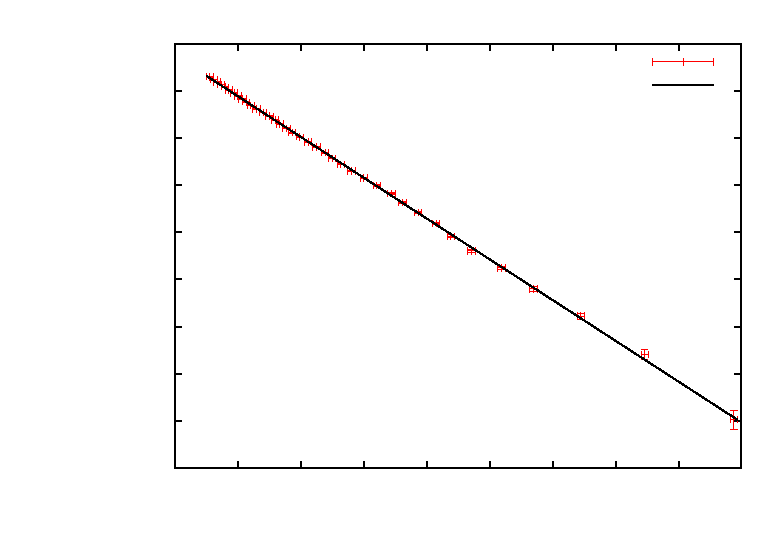
\includegraphics{Erwaermen}}%
    \gplfronttext
  \end{picture}%
\endgroup

	\caption{Arrheniusplot für das Erwärmen}
	\label{fig:mess1}
\end{figure}

\begin{figure}[!htb]
	\centering
	% GNUPLOT: LaTeX picture with Postscript
\begingroup
  \makeatletter
  \providecommand\color[2][]{%
    \GenericError{(gnuplot) \space\space\space\@spaces}{%
      Package color not loaded in conjunction with
      terminal option `colourtext'%
    }{See the gnuplot documentation for explanation.%
    }{Either use 'blacktext' in gnuplot or load the package
      color.sty in LaTeX.}%
    \renewcommand\color[2][]{}%
  }%
  \providecommand\includegraphics[2][]{%
    \GenericError{(gnuplot) \space\space\space\@spaces}{%
      Package graphicx or graphics not loaded%
    }{See the gnuplot documentation for explanation.%
    }{The gnuplot epslatex terminal needs graphicx.sty or graphics.sty.}%
    \renewcommand\includegraphics[2][]{}%
  }%
  \providecommand\rotatebox[2]{#2}%
  \@ifundefined{ifGPcolor}{%
    \newif\ifGPcolor
    \GPcolortrue
  }{}%
  \@ifundefined{ifGPblacktext}{%
    \newif\ifGPblacktext
    \GPblacktexttrue
  }{}%
  % define a \g@addto@macro without @ in the name:
  \let\gplgaddtomacro\g@addto@macro
  % define empty templates for all commands taking text:
  \gdef\gplbacktext{}%
  \gdef\gplfronttext{}%
  \makeatother
  \ifGPblacktext
    % no textcolor at all
    \def\colorrgb#1{}%
    \def\colorgray#1{}%
  \else
    % gray or color?
    \ifGPcolor
      \def\colorrgb#1{\color[rgb]{#1}}%
      \def\colorgray#1{\color[gray]{#1}}%
      \expandafter\def\csname LTw\endcsname{\color{white}}%
      \expandafter\def\csname LTb\endcsname{\color{black}}%
      \expandafter\def\csname LTa\endcsname{\color{black}}%
      \expandafter\def\csname LT0\endcsname{\color[rgb]{1,0,0}}%
      \expandafter\def\csname LT1\endcsname{\color[rgb]{0,1,0}}%
      \expandafter\def\csname LT2\endcsname{\color[rgb]{0,0,1}}%
      \expandafter\def\csname LT3\endcsname{\color[rgb]{1,0,1}}%
      \expandafter\def\csname LT4\endcsname{\color[rgb]{0,1,1}}%
      \expandafter\def\csname LT5\endcsname{\color[rgb]{1,1,0}}%
      \expandafter\def\csname LT6\endcsname{\color[rgb]{0,0,0}}%
      \expandafter\def\csname LT7\endcsname{\color[rgb]{1,0.3,0}}%
      \expandafter\def\csname LT8\endcsname{\color[rgb]{0.5,0.5,0.5}}%
    \else
      % gray
      \def\colorrgb#1{\color{black}}%
      \def\colorgray#1{\color[gray]{#1}}%
      \expandafter\def\csname LTw\endcsname{\color{white}}%
      \expandafter\def\csname LTb\endcsname{\color{black}}%
      \expandafter\def\csname LTa\endcsname{\color{black}}%
      \expandafter\def\csname LT0\endcsname{\color{black}}%
      \expandafter\def\csname LT1\endcsname{\color{black}}%
      \expandafter\def\csname LT2\endcsname{\color{black}}%
      \expandafter\def\csname LT3\endcsname{\color{black}}%
      \expandafter\def\csname LT4\endcsname{\color{black}}%
      \expandafter\def\csname LT5\endcsname{\color{black}}%
      \expandafter\def\csname LT6\endcsname{\color{black}}%
      \expandafter\def\csname LT7\endcsname{\color{black}}%
      \expandafter\def\csname LT8\endcsname{\color{black}}%
    \fi
  \fi
  \setlength{\unitlength}{0.0500bp}%
  \begin{picture}(7200.00,5040.00)%
    \gplgaddtomacro\gplbacktext{%
      \csname LTb\endcsname%
      \put(1386,704){\makebox(0,0)[r]{\strut{} 12}}%
      \put(1386,1286){\makebox(0,0)[r]{\strut{} 12.5}}%
      \put(1386,1867){\makebox(0,0)[r]{\strut{} 13}}%
      \put(1386,2449){\makebox(0,0)[r]{\strut{} 13.5}}%
      \put(1386,3031){\makebox(0,0)[r]{\strut{} 14}}%
      \put(1386,3613){\makebox(0,0)[r]{\strut{} 14.5}}%
      \put(1386,4194){\makebox(0,0)[r]{\strut{} 15}}%
      \put(1386,4776){\makebox(0,0)[r]{\strut{} 15.5}}%
      \put(1518,484){\makebox(0,0){\strut{} 0.0019}}%
      \put(2295,484){\makebox(0,0){\strut{} 0.002}}%
      \put(3072,484){\makebox(0,0){\strut{} 0.0021}}%
      \put(3849,484){\makebox(0,0){\strut{} 0.0022}}%
      \put(4627,484){\makebox(0,0){\strut{} 0.0023}}%
      \put(5404,484){\makebox(0,0){\strut{} 0.0024}}%
      \put(6181,484){\makebox(0,0){\strut{} 0.0025}}%
      \put(6958,484){\makebox(0,0){\strut{} 0.0026}}%
      \put(484,2740){\rotatebox{90}{\makebox(0,0){\strut{}$\ln(\frac{p}{\si{\pascal}})$}}}%
      \put(4238,154){\makebox(0,0){\strut{}$1/T~[\si{1/\kelvin}]$}}%
    }%
    \gplgaddtomacro\gplfronttext{%
      \csname LTb\endcsname%
      \put(5971,4603){\makebox(0,0)[r]{\strut{}Messwerte}}%
      \csname LTb\endcsname%
      \put(5971,4383){\makebox(0,0)[r]{\strut{}Regressionsgerade}}%
    }%
    \gplbacktext
    \put(0,0){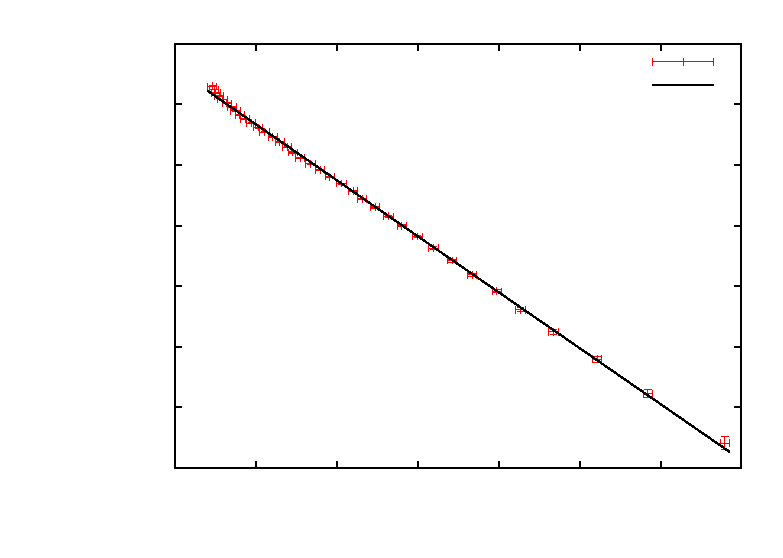
\includegraphics{Abkuehlen}}%
    \gplfronttext
  \end{picture}%
\endgroup

	\caption{Arrheniusplot für das Abkühlen}
	\label{fig:mess2}
\end{figure}

\begin{table}[!htb]
 \centering
 \begin{tabular}{|c|c|c|}
  \hline
  Größe&Erwärmen&Abkühlen\\
  \hline
  m & $(-4326 \pm 13)~\si{\kelvin}$ & $(-4618 \pm 21)~\si{\kelvin}$ \\
  b & $12.07  \pm 0.03$ & $12.54 \pm 0.05$ \\
  \hline
  %$\Lambda_V$ & $(35970 \pm 110)~\si{\joule/\mol}$ & $(38400 \pm 180)~\si{\joule/\mol}$\\
  %\hline
 \end{tabular}
 \caption{Werte aus der linearen Regression der Arrheniusgraphen} 
 \label{tab:regErg}
\end{table}

Dies sind die gewichteten Mittelwerte aus beiden Messungen:
\begin{align*}
 m=(-4407 \pm 11)~\si{\kelvin} \qquad
 b=12.201 \pm 0.024
\end{align*}
Daraus berechnet man die Verdampfungswärme $\Lambda_V$ mit zugehörigem Fehler aus der Fehlerfortpflanzung:
\begin{align*}
 \Lambda_V &= -m\cdot R\\
 \sigma_{\Lambda_V} &= \sigma_m \cdot R\\
 \Lambda_V&=(36640 \pm 100)~\si{\joule/\mol}
\end{align*}
Außerdem kann die Siedetemperatur von Wasser berechnet werden:
\begin{align*}
 T_0 &= -\frac{m}{b}\\
 \sigma_{T_0} &= \sqrt{\left(\frac{\sigma_m}{b}\right)^2+\left(\frac{m\cdot \sigma_b}{b^2}\right)^2}\\
 T_0 &= (361.2 \pm 1.3)\si{\kelvin} = (88.0 \pm 1.3)\si{\celsius}
\end{align*}
Nun berechnen wir noch den Dampfdruck von Wasser bei $T=0\si{\celsius}=273.15\si{\kelvin}$: 
\begin{align*}
 p &= p_0~\exp\left(m\frac{1}{T}+b\right)\\
 \sigma_p &= p~\sqrt{\frac{\sigma_m^2}{T^2}+\sigma_b^2}\\
 p &= (1990 \pm 100)\si{\pascal}
\end{align*}


\subsection{Siedetemperatur auf der Zugspitze}
Hier soll nun die Siedetemperatur des Wassers auf der Zugspitze berechnet werden.
Dort ist der Luftdruck geringer als auf Meereshöhe.
Er berechnet sich nach der \textit{barometrische Höhenformel} \cite[S. 107]{gerthsen}:
\begin{align}
 p(h)=p_0~\exp{\left(\frac{-\rho g h}{p_0}\right)}
 \label{eq:baroHoehenformel}
\end{align}
Wir verwenden hier die Literaturwerte für die Siedertemperatur $T_0$ auf NN und die molare Verdampfungswärme $\Lambda_V$  - nicht die von uns berechneten Werte, da diese eine große Abweichung aufweisen.
Diese Werte und alle weiteren bei dieser Rechnung benötigten sind in der Tabelle \ref{tab:litW} zu finden.
\begin{table}[!htb]
 \centering
 \begin{tabular}{|c|c|}
  \hline
  Größe & Wert\\
  \hline
  T$_0$ & $373.15~\si{\kelvin}$\\
  $\rho$ & $1.29~\si{\kilo \gram/\meter^3}$\\
  g & $9.81~\si{\meter/\second^2}$\\
  R & $8.31~\si{\joule/(\mol.\kelvin)}$\\
  $p_0$ & $1013.25~\si{\hecto \pascal}$\\
  $\Lambda_V$ & $40642 ~\si{\joule/\mol}$\\
  \hline
 \end{tabular}
 \caption{Literaturwerte}
 \label{tab:litW}
\end{table}
Um die Siedetemperatur zu berechnen, setzt man Dampfdruck nach \eqref{eq:Dampfdruck} und Luftdruck nach \eqref{eq:baroHoehenformel} gleich.
\begin{align*}
 \frac{\Lambda_V}{R}\left(\frac{1}{T_0}-\frac{1}{T_S}\right)=-\frac{\rho g h}{p_0}
\end{align*}
Es ergibt sich
\begin{align}
 T_S &= \left(\frac{1}{T_0}+\frac{\rho g h~R}{p_0~\Lambda_V}\right)^{-1}
\end{align}
Für die Höhe der Zugspitze $h=2962~\si{\meter}$ ergibt sich also eine Siedetemperatur des Wassers von $T_S=362.9~\si{\kelvin}=89.8\si{\celsius}$.


\section{Diskussion}
\label{sec:diskussion}
Bei der Verdampfungswärme $\Lambda_V$ ergab sich eine Abweichung zum Literaturwert aus Tab.\ref{tab:litW} von $10\%$ und dieser liegt auch nicht im Fehlerintervall.
Bei der Siedetemperatur kommt es darauf an, ob man die Celsius-Skala oder die Kelvin-Skala zu Grunde legt.
Bei ersterer erhält man eine Abweichung von $12\%$, bei letzterer nur von etwas mehr als $3\%$.
Auch hier liegt der Literaturwert nicht im Fehlerintervall.
Zwar liegen die Messwerte noch in der gleichen Größenordnung, die Abweichungen sind jedoch signifikant.\\
Die gefitteten Geraden der Arrheniusgraphen sehen jedoch gut aus und passen zu den Werten.
Es muss also nach einem systematischen Fehler gesucht werden.
Bei diesem Versuch konnten wir als Praktikanten wenig falsch machen.
Das Ablesen des Druckes war jedoch sehr ungenau und das Manometer musste öfter angestoßen werden, da es zu träge war und keine Druckänderung anzeigte.\\
So muss der Fehler bei den verwendeten Geräten liegen.


%\section{Anhang}

\bibliography{literatur}
\bibliographystyle{babalpha}

\end{document}
